\documentclass[titlepage, a4paper]{article}

\usepackage[swedish]{babel}
\usepackage[utf8]{inputenc}
\usepackage{color}
\usepackage{graphicx}
\usepackage{etoolbox}
\usepackage{stringenc}
\usepackage{pdfescape}

% Sidformat
\usepackage{a4wide}

% Fixa Appendix-titlar
\usepackage[titletoc,title]{appendix}

% Bättre tabeller
\usepackage{tabularx}

% Bättre bildtexter
\usepackage[margin=10pt,font=small,labelfont=bf,labelsep=endash]{caption}

% Enkelt kommando som låter mig attgöra-markera text
\newcommand{\todo}[1] {\textbf{\textcolor{red}{#1}}}

% Nytt \paragraph låter oss ha onumrerade bitar
\makeatletter
\renewcommand\paragraph{\@startsection{paragraph}{4}{\z@}%
{-3.25ex\@plus -1ex \@minus -.2ex}%
{1.5ex \@plus .2ex}%
{\normalfont\normalsize\bfseries}}
\makeatother

\providecommand{\LIPSlogga}{../mall/logga1.png}
\providecommand{\LIPSdatum}{\today}

%% Headers och Footers
\usepackage{fancyhdr}
\pagestyle{fancy}
\lhead{\includegraphics[scale=0.4]{\LIPSlogga}}
\rhead{\ifdef{\LIPSutfardare}{Utfärdat av \LIPSutfardare \\\LIPSdatum}\LIPSdatum}
\lfoot{\LIPSkursnamn \\ \LIPSdokumenttyp}
\cfoot{\thepage}
\rfoot{\LIPSprojektgrupp \\ \LIPSprojektnamn}

%% Titelsida
\newcommand{\LIPSTitelsida}{%
{\ }\vspace{45mm}
\begin{center}
  \textbf{\Huge \LIPSdokument}
\end{center}
\begin{center}
  {\Large Redaktör: \LIPSredaktor}
\end{center}
\begin{center}
  {\Large \textbf{Version \LIPSversion}}
\end{center}
\vfill
\begin{center}
  {\large Status}\\[1.5ex]
  \begin{tabular}{|*{3}{p{40mm}|}}
    \hline
    Granskad & \LIPSgranskare & \LIPSgranskatdatum \\
    \hline
    Godkänd & \LIPSgodkannare & \LIPSgodkantdatum \\
    \hline
  \end{tabular}
\end{center}
\newpage
}

% Projektidentitet
\newenvironment{LIPSprojektidentitet}{%
{\ }\vspace{45mm}
\begin{center}
  {\Large PROJEKTIDENTITET}\\[0.5ex]
  {\small
  \LIPSartaltermin, \LIPSprojektgrupp\\
  Linköpings Tekniska Högskola, IDA
  }
\end{center}
\begin{center}
  {\normalsize Gruppdeltagare}\\
  \begin{tabular}{|l|l|p{25mm}|l|}
    \hline
    \textbf{Namn} & \textbf{Ansvar} & \textbf{Telefon} & \textbf{E-post} \\
    \hline
}%
{%
    \hline
  \end{tabular}
\end{center}
\begin{center}
  {\small
    \ifdef{\LIPSgruppadress}{\textbf{E-postlista för hela gruppen}: \LIPSgruppadress\\}{}
    \ifdef{\LIPSgrupphemsida}{\textbf{Hemsida}: \LIPSgrupphemsida\\[1ex]}{}
    \ifdef{\LIPSkund}{\textbf{Kund}: \LIPSkund\\}{}
    \ifdef{\LIPSkundkontakt}{\textbf{Kontaktperson hos kund}: \LIPSkundkontakt\\}{}
    \ifdef{\LIPSkursansvarig}{\textbf{Kursansvarig}: \LIPSkursansvarig\\}{}
    \ifdef{\LIPShandledare}{\textbf{Handledare}: \LIPShandledare\\}{}
  }
\end{center}
\newpage
}
\newcommand{\LIPSgruppmedlem}[4]{\hline {#1} & {#2} & {#3} & {#4} \\}

%% Dokumenthistorik
\newenvironment{LIPSdokumenthistorik}{%
\begin{center}
  Dokumenthistorik\\[1ex]
  %\begin{small}
    \begin{tabular}{|l|l|p{60mm}|l|l|}
      \hline
      \textbf{Version} & \textbf{Datum} & \textbf{Utförda förändringar} & \textbf{Utförda av} & \textbf{Granskad} \\
      }%
    {%
			\hline
    \end{tabular}
  %\end{small}
\end{center}
}

\newcommand{\LIPSversionsinfo}[5]{\hline {#1} & {#2} & {#3} & {#4} & {#5} \\}

% Kravlistor
\newenvironment{LIPSkravlista}{
	\center
		\tabularx{\textwidth}{| p{1.2cm} | p{1.9cm} | X | c |}
			\hline
			\textbf{Krav} & \textbf{Förändring} & \textbf{Beskrivning} & \textbf{Prioritet} \\\hline
}
{
		\endtabularx
	\endcenter
}

\newcounter{LIPSkravnummer}
\addtocounter{LIPSkravnummer}{1}
\newcommand{\LIPSkrav}[4][Krav \arabic{LIPSkravnummer}]{{#1} & {#2} & {#3} & {#4} \stepcounter{LIPSkravnummer}\\\hline}


% Leveranskravlistor
\newenvironment{LIPSleveranskravlista}{
	\center
		\tabularx{\textwidth}{| p{1.2cm} | p{1.9cm} | X | X |}
			\hline
			\textbf{Krav} & \textbf{Förändring} & \textbf{Beskrivning} & \textbf{Deadline}\\\hline
}
{
		\endtabularx
	\endcenter
}

\newcounter{LIPSleveranskravnummer}
\addtocounter{LIPSleveranskravnummer}{1}
\newcommand{\LIPSleveranskrav}[4][Krav \arabic{LIPSkravnummer}]{{#1} & {#2} & {#3} & {#4} \stepcounter{LIPSkravnummer}\\\hline}


% Milstolps-lista
\newenvironment{LIPSmilstolpar}{
	\center
		\tabularx{\textwidth}{| p{1.2cm} | X | l |}
			\hline
			\textbf{Nr} & \textbf{Beskrivning} & \textbf{Datum} \\\hline
}
{
		\endtabularx
	\endcenter
}

\newcounter{LIPSstolpnummer}
\addtocounter{LIPSstolpnummer}{1}
%\newcommand{\LIPSmilstolpe}[3][Krav \arabic{LIPSstolpnummer}]{{#1} & {#2} & {#3} \stepcounter{LIPSstolpnummer}\\\hline}
\newcommand{\LIPSmilstolpe}[3]{{#1} & {#2} & {#3} \\\hline}

% Aktivitets-lista
\newenvironment{LIPSaktivitetslista}{
	\center
		\tabularx{\textwidth}{| p{0.3cm} | X | c | c | c |}
			\hline
			\textbf{Nr} & \textbf{Beskrivning} & \textbf{Beroende av} & \textbf{Timmar} & \textbf{datum} \\\hline
}
{
		\endtabularx
	\endcenter
}

\newcounter{LIPSaktivitetsnummer}
\addtocounter{LIPSaktivitetsnummer}{1}
% \newcommand{\LIPSaktivitet}[4][\arabic{LIPSstolpnummer}]{{#1} & {#2} & {#3} & {#4} \stepcounter{LIPSstolpnummer}\\\hline}
\newcommand{\LIPSaktivitet}[5]{{#1} & {#2} & {#3} & {#4} & {#5}\\\hline}

% Mall för mötesprotokoll
\newenvironment{projektmote}[2]{
  {\ }\vspace{5mm}

  \centerline{\textbf{\Huge #1}}
  \vspace{2mm}
  \centerline{\LARGE #2}
  \vspace{10mm}

  \begin{itemize}
}
{
  \end{itemize}
}

\newcounter{paragrafnummer}
\addtocounter{paragrafnummer}{1}
\newcommand{\paragraf}[1]{\item{\textsection \arabic{paragrafnummer}. {#1}}\addtocounter{paragrafnummer}{1}}

% Mall för Statusrapport
\newenvironment{statusrapport}{
  \center
    \tabularx{\textwidth}{| p{0.4cm} | X | X | p{14.5mm} | p{13.5mm} | p{16.5mm} | p{16.5mm} |}
    \hline
    \textbf{Nr} & \textbf{Aktivitet} & \textbf{Beroenden} & \textbf{Planerad tid} & \textbf{Nedlagd tid} & \textbf{Planerad klar} & \textbf{Beräknat klart} \\\hline
}
{
    \endtabularx
  \endcenter
}

\newcommand{\aktivitetstatus}[7]{{#1} & {#2} & {#3} & {#4} & {#5} & {#6} & {#7} \\\hline}	% Importera generella layout-strukturer

% Information nödvändig för generella layout-strukturer
\newcommand{\LIPSredaktor}{Martin Söderén}
\newcommand{\LIPSversion}{0.1}
\newcommand{\LIPSdokument}{Optimering av matrisbibliotek i C}
\newcommand{\LIPSdokumenttyp}{Kandidatrapport}
\newcommand{\LIPSgranskatdatum}{-}
\newcommand{\LIPSgranskare}{Martin Söderén}
\newcommand{\LIPSgodkannare}{Andreas Runfalk}
\newcommand{\LIPSgodkantdatum}{-}
\newcommand{\LIPSkursnamn}{TDDD77}
\newcommand{\LIPSprojektnamn}{Prediktionsreglering}
\newcommand{\LIPSprojektgrupp}{Grupp 2}
%\newcommand{\LIPSgruppadress}{\todo{Ta bort}}
\newcommand{\LIPSartaltermin}{VT, 2015}
\newcommand{\LIPSgrupphemsida}{http://pum-2.ida.liu.se/}
\newcommand{\LIPSkund}{SAAB}
\newcommand{\LIPSkundkontakt}{Daniel Simon}
\newcommand{\LIPSkursansvarig}{Kristian Sandahl}
\newcommand{\LIPShandledare}{Andreas Runfalk}
% Dokument-specifika paket
\usepackage{tabularx}
\usepackage{pdfpages}
\usepackage{tikz}
\usepackage{float}
\usepackage{graphicx}
\usepackage{algorithm}
\usepackage{algpseudocode}
\usepackage{natbib}
\usepackage{listings}
\usepackage{mathtools}
\usetikzlibrary{shapes, arrows}

\pagenumbering{roman}

\DeclareGraphicsRule{.0.pdf}{pdf}{*}{}

\begin{document}

\LIPSTitelsida


\newpage
\tableofcontents	%Innehållsförteckning
\newpage
\pagenumbering{arabic}
\section{Inledning}
Byggsystem är en viktig men ofta förbisedd komponent i en utvecklares verktygslåda. Byggsystemet ansvarar för att automatiskt göra om källkoden till körbara filer utan att utvecklaren ska behöva komma ihåg långa kompilatorkommandon, sökvägar till programbibliotek och liknande. Ett bra byggsystem medför en rad fördelar, ökad produktivitet och förbättrade möjligheter till testning för att nämna några.

I den här rapporten kommer två olika byggsystem att jämföras med projektet ''Prediktionsreglering'' som utgångspunkt. Projektets befintliga byggsystem implementerat i Make kommer att ställas mot ett nytt implementerat i SCons. 

\subsection{Syfte}
Då min roll i projektet är utvecklingsledare tog jag beslutet om att använda Make som byggsystem tidigt i projektets gång. Detta då Make finns förinstallerat på både Mac och de flesta Linuxdistributioner. Syftet med den här rapporten är att utreda ett alternativ till Make och om några fördelar för projektet finns.

\subsection{Frågeställning}

\begin{enumerate}
\item Vilket av de två byggsystemen har bäst prestanda?
\item Vilket byggsystem är lättast att använda och utveckla?
\item Hur hade projektet påverkats av ett annat val av byggsystem?
\end{enumerate}

\subsection{Avgränsningar} \label{avsnitt:avgransningar}
Rapporten kommer återspegla resultat för projektet ''Prediktionsreglering'' som består av \todo{?} källkodsfiler och \todo{?} dokumentfiler. Projektets kod ska kunna byggas och exekveras på både Linux, Mac och Windows. Resultaten skulle kunna se annorlunda ut med ett projekt av annan storlek och andra krav. Byggsystemen kommer endast att jämföras på punkten att kompilera och länka kod, ej köra tester eller generera dokument, detta på grund av tidsbrist.

\subsection{Bakgrund}
Jag har under kursen Kandidatprojekt i programvaruutveckling haft rollen som teamledare för en grupp bestående av sex andra studenter vid Linköpings universitet. Som teamledare har man i detta fall ansvar för en rad olika administrativa uppgifter vilket bland annat innebär ansvar för projektets framgång och uppfyllande av de krav som finns uppsatta. Under denna process väcks många frågor kring hur väl den antagna rollen uppfylls jämfört med arbetslivet vilket lett till denna jämförelse mellan mina prestationer som teamledare och de 'best practises' som kan tillämpas.
\newline \newline
Det projekt som har genomförts är att skapa ett program som löser ett optimeringsproblem. Till detta program hör dels en lösare, ett grafiskt gränssnitt och en parser som översätter optimeringsproblemet till C-kod för att lösaren ska kunna lösa problemet. 
\section{Teori}
Denna rapport har egentligen två huvudbegrepp, 'best practice' och teamledare. 'Best practices' är enligt Oxfords engelska uppslagsverk som "Commercial or professional procedures that are accepted or prescribed as being correct or most effective" \cite{OD}. Löst översatt till svenska betyder detta kommersiella eller professionella tillvägagångssätt vilka är accepterade och föreskrivna som korrekta och mest effektiva. Med andra ord är en 'best practice' det sätt en person på bäst sätt kan utföra en uppgift vilket i fallet som teamledare innebär att genomföra rollen på bästa sätt \cite{itSMF}. 
\newline \newline
Det andra begreppet som är av stor betydelse i denna rapport är som tidigare nämnts teamledare. En teamledare kan beskrivas på många sätt men en generell beskrivning är att en teamledare är en gruppmedlem som kan ha viss bestämmanderätt över gruppen men detta är ingen nödvändighet. En teamledare kan antingen vara permanent utsedd eller utsedd under kortare perioder där rollen vandrar mellan olika gruppmedlemmar. Oavsett om teamledaren är permanent utsedd eller inte har denne ett ansvar att representera gruppen utåt samt uppåt vilket betyder att denne kan vara ansvarig gentemot eventuella chefer men teamledaren har även ett ansvar gentemot gruppen i sig. Detta ansvar innebär att teamledaren ska lösa konflikter inom gruppen samt koordinera dess arbete för att uppnå uppsatta mål mål \cite{BD}. 
\newline \newline
När det gäller själva ledarskapet finns det ett antal olika modeller eller stilar. En av dessa togs fram av Kurt Lewin tillsammans med sin forskargrupp under 1930-talet och heter därefter Lewin's Leadership Syles. I studien undersöktes skolbarn som genomförde olika projekt för att se vilka typer av ledarroller som barnen antog. Det man kom fram till var att det fanns tre stilar. En auktoritär, en deltagande eller demokratisk och en delegerande \cite{KAC} vilket illustreras av Figur ~\ref{fig:Lewin}. 
\begin{figure}[h]
\centerline{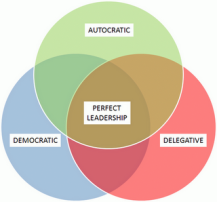
\includegraphics{adam-tex/graphic/leadership}}
\caption{Lewin's Leadership Style}
\label{fig:Lewin}
\end{figure}
\newline
Figuren visar tre cirklar vilka representerar de olika ledarstilarna och att en ledare inte nödvändigtvis behöver tillämpa en av de tre stilarna utan kan tillämpa flera av dem samtidigt. Detta innebär att en riktigt bra ledare, oavsett vilken typ av ledare det rör sig om, har delar av alla tre stilarna för att vid behov kunna använda den som är mest lämpad för situationen. Dock är detta, som tidigare nämnts, en av många modeller för ledarskap men har valts som exempel för att den är generell och lätt att tillämpa på rollen som teamledare.
\section{Metod}
%Informationen kommer från en kombination av det som står på nätet och i böcker med mina egna erfarenheter från tidigare större programmeringsprojekt.
Under utvecklandet av arkitekturen 

 

\section{Resultat}	
	Följande del beskriver hur arbetet med efterforskningen gick samt hur testen utfördes.
	\subsection{Efterforskning}
	Det finns otroligt mycket information om mjukvarutestning men samtidigt är ämnet ganska vagt då testning beror så mycket på just vad som ska testas. I vårt projekt visade det sig att ''Black Box''-testning var den metod som överlägset lämpade sig bäst. ''Black Box'' går ut på att man sätter en ''svart låda'' över det som ska testas, så att man endast kan se in- och utdatan. Sedan kollar man ifall udatan är den förväntade. ''Black Box'' anses bra i detta projekt eftersom hela Quadopt är uppbyggd utav många små funktioner och resultateten som de ska ge tillbaka är oftast kända på förhand. Ett exempel på detta är matrisaritmetiken där resultatet, av till exempel en multiplikation, går att räkna ut ganska enkelt på papper. Enligt ''The Art of Software Testing'' ska dessa test utgå ifrån kravspecifikationen och andra dokument som beskriver vad produkten ska ha för funktionalitet. Boken beskriver också ''Black Box'' som en utmattande testteknik. Med det menar de att man borde testa alla möjliga indata till den svarta lådan och se så att svaren stämmer. Detta är precis som det står i boken i praktiken omöjligt. Speciellt i vårt projekt där det enda som begränsar antalet olika sätt en matris, bestående utav tal, kan se ut på är datorns minne. \newline
I projektet fanns dock ofta behovet av se en funktions lösningsgång, och då är ''Black Box'' en väldigt dålig metod. En metod som då lämpar sig bättre är ''White Box'' testning, som innebär att man kollar på den interna strukturen i en funktion. Därefter kan man kolla, efter vald indata, om lösningsgången är den väntade. I ''The Art of Software Testing'' står det att även denna metod kan problematisk då antalet lösningsgångar kan vara väldigt många. För att se om det ens är rimligt att utföra dessa test kan man kolla på funktionens cyklomatiska komplexitet. Cyklomatisk komplexitet innebära att man gör en graf över funktionen där de möjliga stadierna i lösningsgången är noder, och de möjliga lösningsvägarna är bågar. I ''Structured testing'' \citep{structest} står det att om denna komplexitet är för stor ökar antalet fel som programmeraren gjort väldigt fort, och samtidigt blir det i stort sett omöjligt att uföra några ''White Box''-test då fel kan uppstå på så många ställen. \\ 	
För att säkerställa projektets krav behövdes bara en testmetod till, och det var en metod för att mäta prestanda. Den som valdes var ''Load testing'' som innebär att man belastar programmet med mycket data och så kollar man på hur bra det fungerar. I projektets fall gavs lösaren många problem och kollade på hur fort det gick i förhållande till andra lösare. \newline	
Det skulle kunnat varit så att GUI:t hade haft högre prioritet än vad det hade. I det fallet hade olika typer av UX- användartest varit nödvändiga för att kvalitetsssäkra produkten. Men eftersom GUI:t beställdes utifrån kundens personliga behov, var det tydligt definierat redan från början att det var av låg prioritet. 
	
	\subsection{Praktik}
	Som beskrivet tidigare finns det i stort sett oändligt många kombinationer av in- och utdata.	För att då kunna utföra ''Black Box''-testerna behövdes antalet testfall reduceras. Detta åstakoms genom att ha möten med kunden som klargjorde att indata till programmet alltid skulle vara giltig. Det reducerade antal testfall enormt mycket, men som beskrivet i resultatet av efterforskningen finns det även väldigt mycket giltig indata. Exempelvis för matrisaritmetiken. Dessa test gick också att reducera genom att de flesta operationer är triviala och endast kräver numeriska test såsom nolldivision och flyttalsfel. Genom att även utnyttja ''White Box''-tekniken gick det att utforma olika ''Black Box''-test som tog olika vägar genom koden och på så sätt bara skapa ett test för varje väg. Denna teknik utnyttjades endast på mindre funktioner såsom moduler för att antalet olika fall skulle begränsas till något som var rimligt. \newline
	För lösaren gick det att applicera samma metod, eftersom dess funktionalitet bygger mycket på underliggande funktioner. Det som skilde sig gentemot småfunktionerna var att nu behandlades oftast rader eller kolumner i matriser istället för enskillda element. Detta ledde till att de flesta test kollade på kanterna utav det tillåtna området. Alltså kunde ett test vara att försöka hämta ut en radvektor på rad -1 ur en matris, vilket skulle vara ogiltigt.\newline
Vid granskning av testresultat från git, Travis (verktyg för Continuous integration) och gruppmedlemmar visade det sig att majoriteten fel av bestod utav två typer: ''Assertion''s som misslyckats och ''Segmentations fault''. En ''Assertion'' är ett test inuti koden som avbryter exekveringen om testet inte går bra. ''Seqmentation fault'' är ett programmeringsfel som resulterat i en ogiltig läsning eller skrivning till minnet. Felen som uppstod var väldigt utspridda och olika. Det som de flesta hade gemensamt var dock att de låg på en låg nivå, alltså i bottenfunktionerna. \newline	
	För att testa algoritmens hastighet stötte gruppen på oväntade problem, lösarna var för snabba.	Då varje testkörning tog 0.00 sekunder för alla lösarna förutom MATLAB behövdes testen köras många gånger för att se en tydlig skillnad. Anledningen till att MATLAB är långsammare är för att den är oerhört generell men förmodligen inte gjorts med fokus på att vara snabb. Gurobi är snabb eftersom dens enda uppgift är att lösa sådana här problem och har arbetats på under lång tid. Vår algoritm är snabb eftersom den inte är generell, alltså bryr vi oss inte om vissa specialfall som vi aldrig kommer stöta på. \newline
	För att då testa deras prestanda fick lösarna lösa olika optimeringsproblem många gånger, ofta upp emot 1000 gånger, för att kunna skilja deras egentliga hastighet. Att köra testen på vår lösare och i matlab var enkelt då vi hade funktionalitet för att konvertera matriser från MATLABs definition till vår, och vice versa. Däremot så var det krångligare i gurobi eftersom tiden som var allokerad för utbildning av programmet var begränsad. Det tvingade gruppen till att mata in problemet på ekvationsform vilket gjorde att gruppmedlemmarna var tvungna att köra endast små tester. Redan vid problem med fler än 10 bivillkor skulle det ta väldigt lång tid att konvertera och mata in problemet. \newline
	
	
	\subsection{Enhetstester}
	Under projektet har många enhetstest skrivits (framförallt för matrisbiblioteket). Dessa test har skrivits innan och under kodningen och sedan utförts direkt efter att koden blivit klar. Det som var intressant med dessa test var mängden av fel som upptäcktes direkt. Det ledde till att utvecklingen blev mycket effektiv då fel kunde åtgärdas direkt.
	
	\subsection{Integrationstester}
	De modultester som planerades och utfördes under projektet var framförallt lösarens funktioner. Modulerna var uppbyggda utav sammansättningar av enheter från matrisbiblioteket och andra strukturer. Dessa test utfördes vanligtvis samtidigt som implementeringen pågick. Detta för att hela tiden se till att rätt protokoll och gränsnitt användes.\\
De systemtester som utförts är tester utav lösaren och sublösaren. Dessa ansågs vara tillräcklig komplexa för att ses som system. 
	
	
	\subsection{Acceptanstester}
	De acceptanstester som utförts under projektet är framförallt prestandatester. Detta för att det enda kravet lösaren hade var att den skulle vara ungefär lika snabb som den kommersiella lösaren gurobi. De delar som testats då var underfunktioner till lösaren, såsom matrisbiblioteket och subproblemslösaren.
	
	\subsection{Misstag}
	Det hände att vissa modul- och systemtester skedde innan de underliggande enheterna blivit testade. Ett exempel på det är lösaren som vi var ivriga att få igång och började testa tidigt. Då den inte fungerade korrekt gjorde detta att det tog lång tid att hitta felet som förmodligen hade upptäckts mycket snabbare om bara rätt testprocess hade använts.
	
	
\section{Diskussion}
\subsection{Resultat}
Att det tog hela projekttiden för att gruppens samtliga medlemmar skulle känna att de behärskade {\LaTeX} någorlunda bra förefaller inte som någon överraskning. Även om man behärskar andra programmeringsspråk är det fortfarande en nytt språk som ska läras. Enligt \citep{latexandfriends} är {\LaTeX} ett svårt språk som kan ta flera månader att behärska. 
\newline
\newline
Inlärningen av {\LaTeX} var inte kontinuerlig under projektets gång. Det skedde nästan enbart i projektets förstudie och slutskede därför det var då flest dokument skulle inlämnas. Om inlärningen hade varit kontinuerlig hade samtliga medlemmar med största sannolikhet kunnat behärska {\LaTeX} tidigare.
\newline
\newline
Användandet av {\LaTeX} på Windows innebar en del problem. Programmet TeXMaker kunde inte installera en del paket som kunde installeras på de andra plattformarna. Den hade även en del störande moment som att den alltid frågade om lov när nya paket skulle installeras.  
 
\subsection{Metod}
Då det fanns andra grupper som gjorde liknande projekt samtidigt som oss kunde studien även ha utförts på dessa grupper för att få ett bredare perspektiv. 
\section{Slutsatser}
\todo{Vad var snabbast,lättast etc} \\
\todo{Varför är byggsystem så annorlunda gentemot vanlig programmering - deklarativt!} \\


\bibliographystyle{plain}
\bibliography{martin-tex/mybib}{}

\end{document}